\newpage


\section{Convolutional Neural Networks (CNNs)}
\label{sec:convolutional-neural-networks-(cnns)}

Convolutional Neural Networks introduce a powerful tool for defining models that perfectly fits image elaboration.
This tool, which gives the name to the networks, is the \textbf{Convolution layer}.

\paragraph{Convolution}
It applies homonymous mathematical operation by combining two functions to produce a third one, in the discrete case:
\[(f\ast g)(n) = \sum f(m)g(n-m)\]
Where, in the context of images, $f$ could represent an image and $g$ a kernel.

More intuitively the kernel combines the pixels of images in a window to generate altered values based on the neighborhood.
In neural network this is not any different as the weighted inputs are convoluted by the kernel specification.

In image processing convolution is a basic element for many tasks, and it becomes powerful in neural networks
as the learning process defines the weights for the kernel matrices.
The power in applying convolutions to the data is that it can alter information contained to better show features of
the image, which is what we often see in shown examples, from simple lines to complex shapes the deeper the convolutions.

In keras this is obtained by the \textbf{Conv2D}\cite{con2d} layer object, such as:
\begin{verbatim}
x = keras.layers.Conv2D(
    filters=64, kernel_size=(3,3), padding="same", activation="relu"
)
\end{verbatim}

\paragraph{Pooling}
In order to reduce the amount of parameters and improve generalization one can use the \textbf{Pooling} layer.
The pooling operation simply down-samples the feature map of the data. In keras this is achived by any implementation
of the pooling operation. As empirical performance between the various methods\cite{bieder2021comparison}
doesn't favor any precise method, the \textbf{MaxPooling2D}\cite{maxpooling2d} was used.

\\

\paragraph{}
For a long time CNNs have been the state of the art for various fields involving machine learning, including Computer Vision.
Now that transformers have become popular CNNs might have been outclassed but the question is still open for debate.\cite{wang2023cnns}
Besides being very effective the fact that they are both easier to train and less memory constraining were other good reasons
to favor CNNs instead of the simple MLPs approach.

\subsection{Model Structure}
% todo finish with images

\paragraph{First Model}
For the first model(\ref{fig:custom_cnn}) the approach was to apply more than one convolution layer as they better
capture more complex features. By downsampling the image we also reduce the power of representation of each layer.

A good rule for designing CNN, confirmed by empirical evidence on VGG and ResNet, is to increase the number of filters
in deeper layers as the down-sampling drastically reduces the power of representation of the network.
This rule was applied to the definition of the model.

For the first training procedure the model had no image augmentation procedure defined and a fixed number of epochs, this
led to overfitting the training set with an 88\% accuracy on the test set with a very high loss of 0.6591.

% todo riferimento a coso
To avoid overfitting we apply the dataset augmentation as defined in\ref{fsfs}.
This resulted in a better model that had $acc=89.10\%$ and a $l=0.2536$ on test with fixed learning epochs.
We now use K-fold-CV and early stopping to estimate the expected performance of the predictor before re-training a new one.
The results of the procedure are reported in \ref{tab:kfoldcnn}.


\begin{figure}[h]
    \centering
    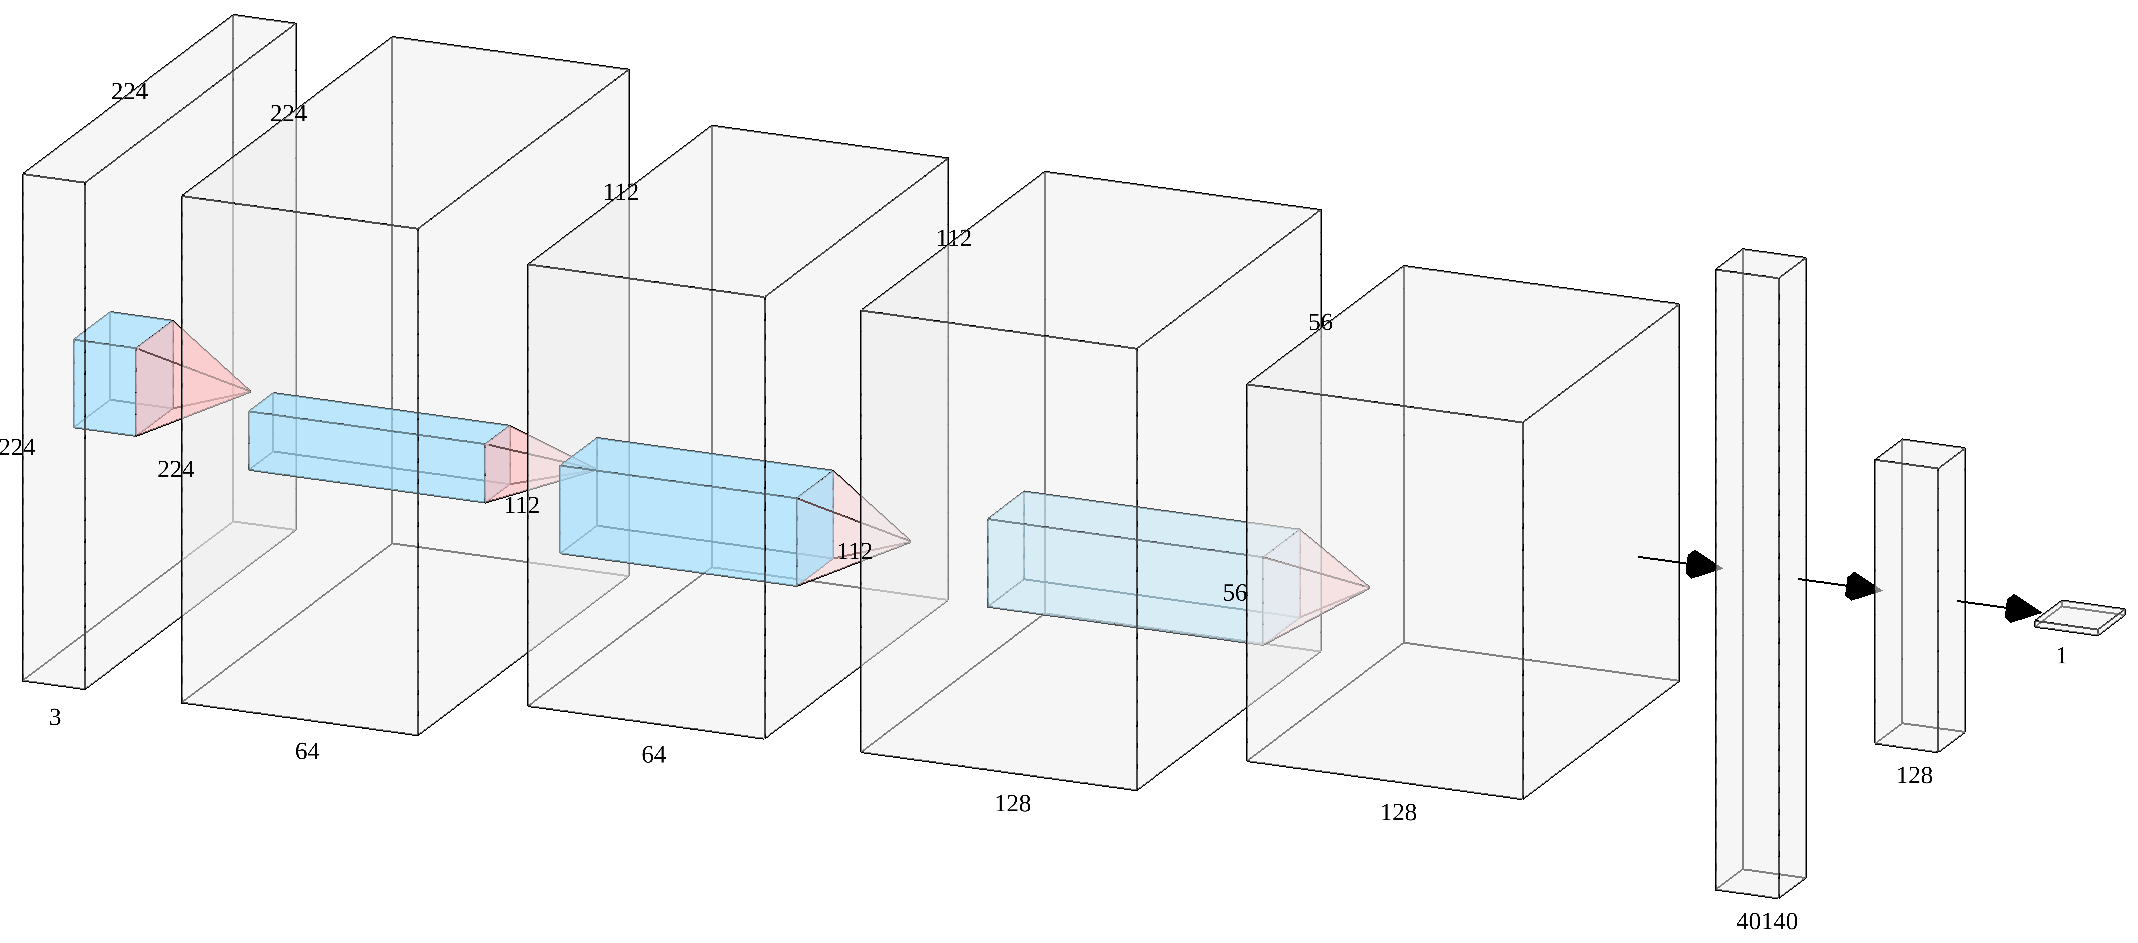
\includegraphics[scale=0.15]{imgs/custom-cnn-one}
    \caption{
        Graphical representation of the first CNN model. (Not in scale)\\
        \textit{Image generated via the NN-SVG tool}
    }\label{fig:custom_cnn}
\end{figure}

\paragraph{Second Model}

To reduce overfitting on the first model we tried defining a model with fewer parameters.
The structure of the model is defined in \ref{fig:second-conv-net-structure}
and has, only on the first Convolution layer, a wider kernel of size $(5\times5)$ in the hope of the network to capture a broader context.

For this network the learning parameters have not been fine tuned as during the designing tests it performed
on par with the other model. The optimal configuration for the first conv network was instead used.
To estimate the network performance, we ran k-Fold-CV. The results are reported in the table(\ref{tab:kfoldcnn}).

The final model is in line with the expected performance as it measured $acc=89.27\%$ and $l=0.1073$
on the test set. If we tuned the training hyperparameters specificially for this architecture we might have gotten better model.


\begin{figure}
    \centering
    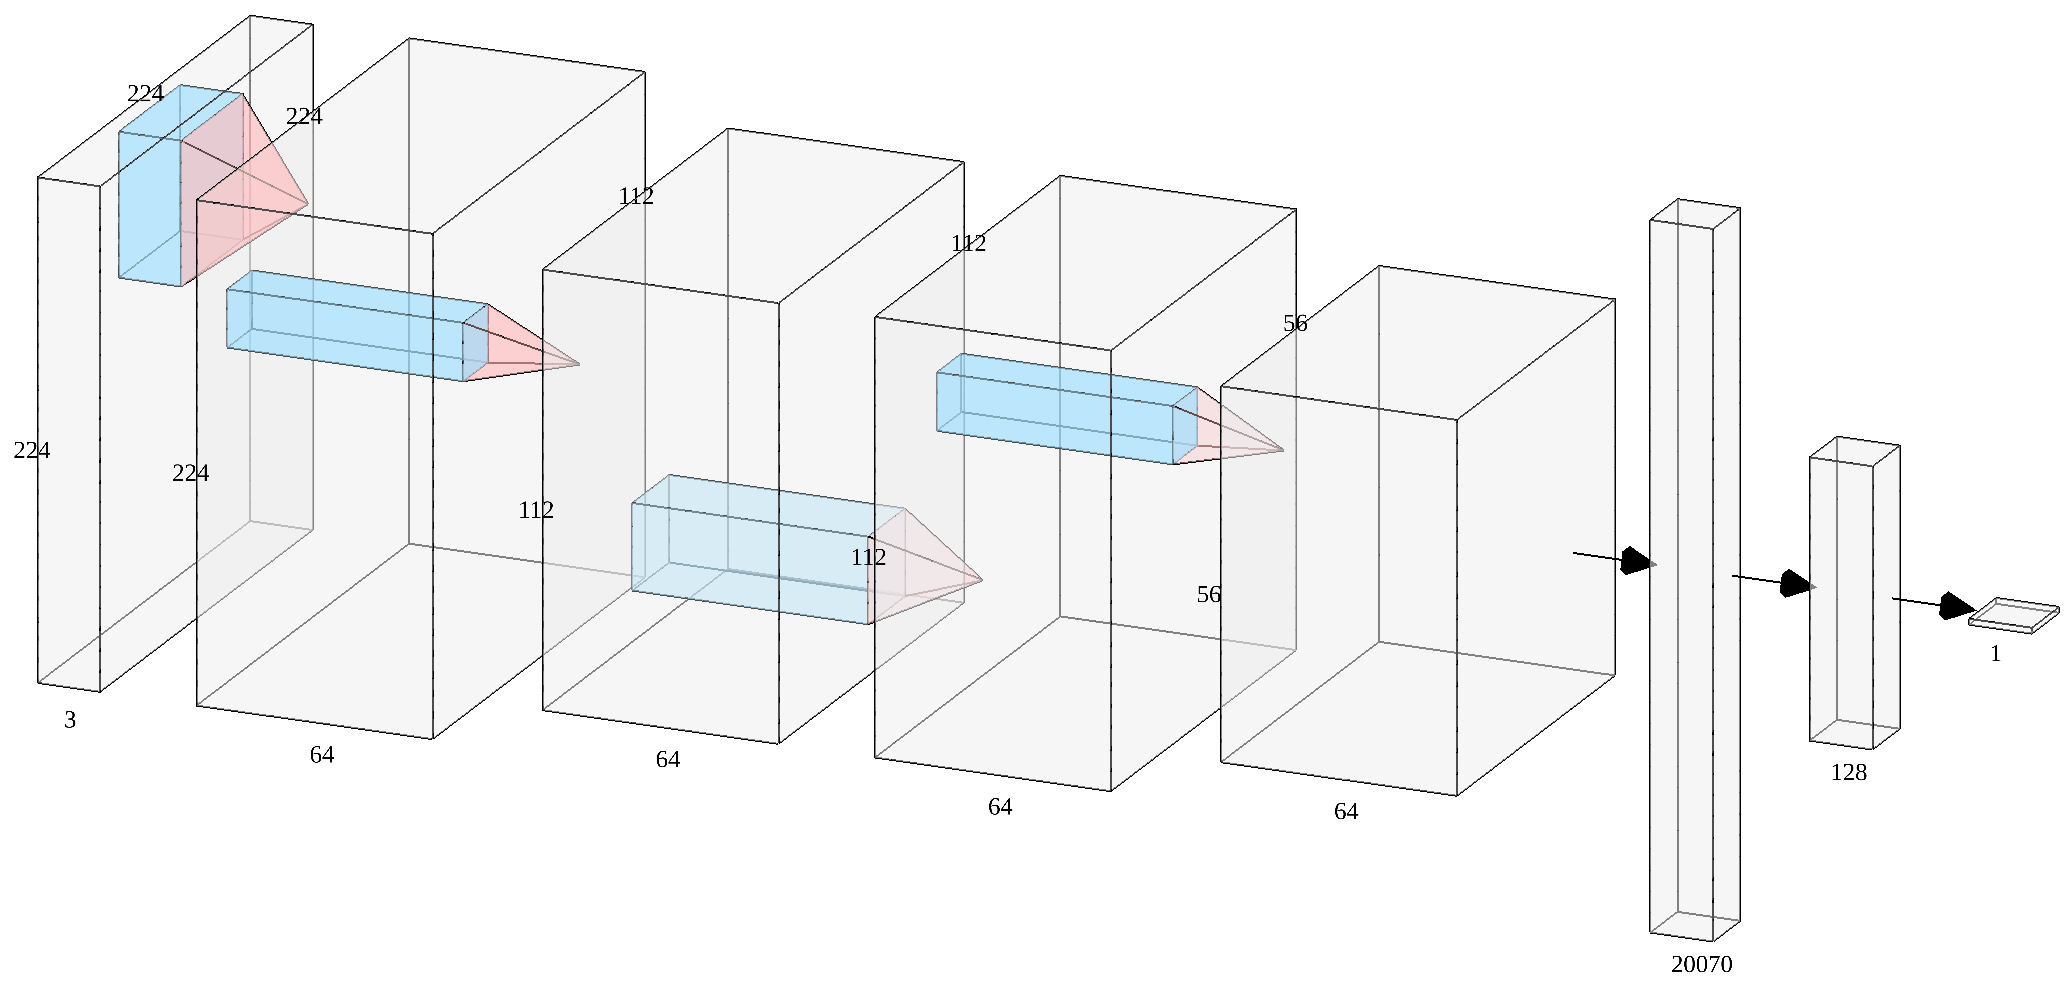
\includegraphics[scale=0.15]{/home/jacopo/PycharmProjects/muffin-stat-project/report/imgs/second-conv-net-structure}
    \caption{
        Graphical representation of the second CNN model. (Not in scale)\\
        \textit{Image generated via the NN-SVG tool}
    }
    \label{fig:second-conv-net-structure}
\end{figure}


\begin{table}
    \centering
    \begin{tabular}{ | c | c | c | }
        \hline
        $k$ & $accuracy$ & $l_{0-1}$ \\
        \hline\hline
        0   & 0.8666     & 0.1334    \\
        \hline
        1   & 0.9029     & 0.0971    \\
        \hline
        2   & 0.8707     & 0.1293    \\
        \hline
        3   & 0.8935     & 0.1065    \\
        \hline
        4   & 0.8808     & 0.1192    \\
        \hline
        \hline
        avg & 0.8829     & 0.1171    \\
        \hline
    \end{tabular}
    \quad
    \begin{tabular}{| c | c | c |}
        \hline
        $k$ & $accuracy$ & $l_{0-1}$ \\
        \hline\hline
        0   & 0.8910     & 0.1090    \\
        \hline
        1   & 0.8970     & 0.1030    \\
        \hline
        2   & 0.8377     & 0.1623    \\
        \hline
        3   & 0.8986     & 0.1014    \\
        \hline
        4   & 0.8986     & 0.1014    \\
        \hline
        \hline
        avg & 0.8846     & 0.1154    \\
        \hline
    \end{tabular}
    \caption{
        Left the first model's \textit{k-fold-CV} estimates, right the second one's.
    }

    \label{tab:kfoldcnn}
\end{table}

\subsubsection{Autotuned CNN}
While the CNN yield not bad results given their simplicity a better structure could be sure identified.
Instead of going on by trial and error we wanted to auto-tune the architecture of the network itself.

In order to do achieve this result while still testing a good amount of combinations, the search space
was confined to the following variables:
\begin{description}
    \item [convolutional\_layers] The amount of $(CONV \rightarrow POOL)$ layers to build.\\
    For each of these, the pooling layer parameters were fixed.
    \item[filters\_i] Number of filters, a power of two from 16 to 256.\\
    The setting is referred to the specific convolution layer $i$
    \item[kernel\_i] The square size of the kernel chosen from the set of values: $\{3,5\}$.
    The setting is referred to the specific convolution layer $i$
    \item[hidden\_layers] Number of dense layers that follow the convolutional ones
    \item[units\_i] Number of units for the dense layer $i$
\end{description}

The optimization process has run for a total of 40 iterations and resulted in various models with a close performance.
From the results a trend indicates that networks with more convolutional layers generally lead to better results.

\paragraph{Auto-tuned Model}

The best performing model is of the characterized by 4 convolution layers followed a flattening layer by 2 dense layers.
At top of the network a single dense neuron layer with sigmoid activation is put for final classification.
The structure can be seen in the shown image \ref{fig:5_autotuned_netw_structure}.

The learning parameters for the CNN were also fine-tuned which led to a final model with TODO acc e loss
which is on par with what we expect given the k-fold estimates.

% struttura del coso
\begin{figure}
    \centering
    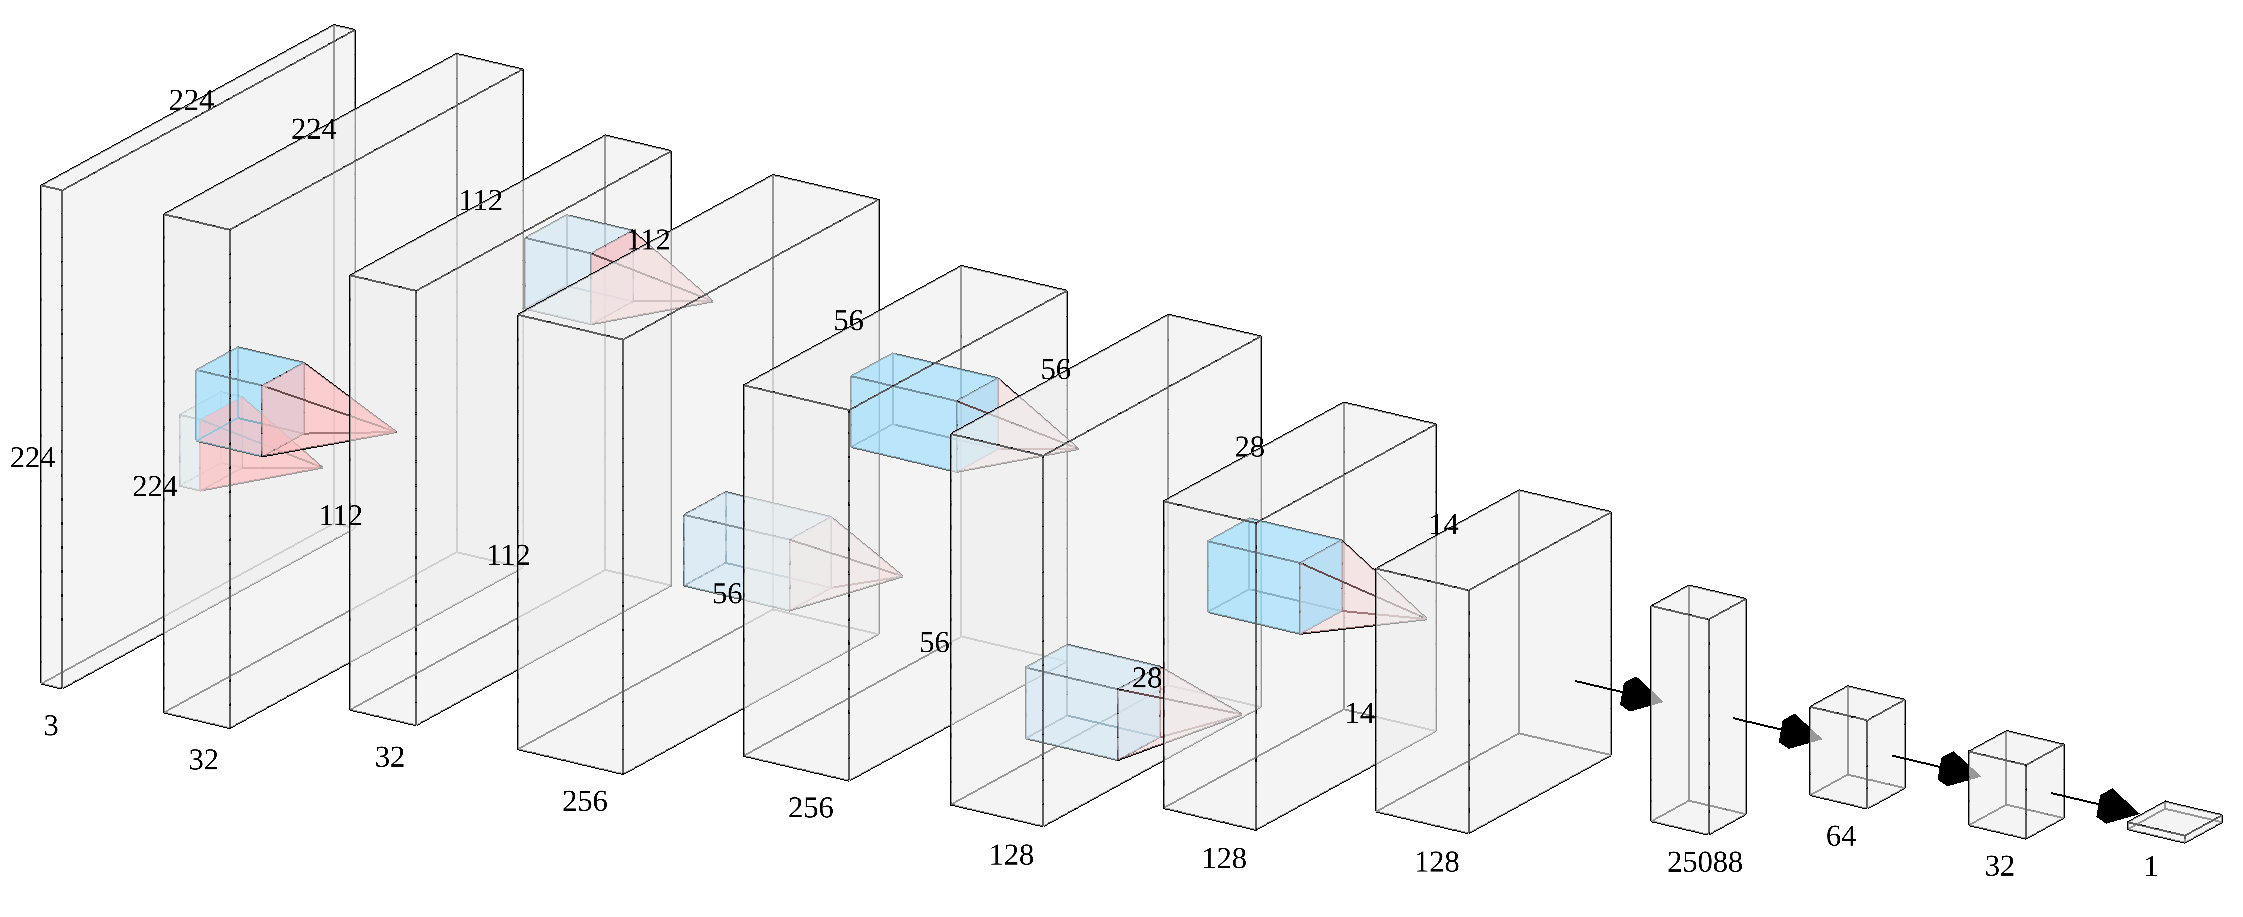
\includegraphics[scale=0.15]{/home/jacopo/PycharmProjects/muffin-stat-project/report/imgs/5_autotuned_netw_structure}
    \caption{
        Graphical representation of the autotuned CNN model structure. (Not in scale)\\
        \textit{Image generated via the NN-SVG tool}
    }
    \label{fig:5_autotuned_netw_structure}
\end{figure}
\begin{table}
    \centering
    \begin{tabular}{| c | c | c |}
        \hline
        $k$ & $accuracy$ & $l_{0-1}$ \\
        \hline\hline
        0   & 0.9459     & 0.0270    \\
        \hline
        1   & 0.9139     & 0.0431    \\
        \hline
        2   & 0.9527     & 0.0237    \\
        \hline
        3   & 0.9645     & 0.0178    \\
        \hline
        4   & 0.9358     & 0.0321    \\
        \hline
        \hline
        avg & 0.9426     & 0.0287    \\
        \hline
    \end{tabular}
    \caption{
        Left the first model's  \textit{k-fold-CV} estimates, middle second,  right the thrid one.
    }

    \label{tab:kfoldbestcnn}
\end{table}
